%% BioMed_Central_Tex_Template_v1.06
%%                                      %
%  bmc_article.tex            ver: 1.06 %
%                                       %

%%IMPORTANT: do not delete the first line of this template
%%It must be present to enable the BMC Submission system to
%%recognise this template!!

%%%%%%%%%%%%%%%%%%%%%%%%%%%%%%%%%%%%%%%%%
%%                                     %%
%%  LaTeX template for BioMed Central  %%
%%     journal article submissions     %%
%%                                     %%
%%          <8 June 2012>              %%
%%                                     %%
%%                                     %%
%%%%%%%%%%%%%%%%%%%%%%%%%%%%%%%%%%%%%%%%%


%%%%%%%%%%%%%%%%%%%%%%%%%%%%%%%%%%%%%%%%%%%%%%%%%%%%%%%%%%%%%%%%%%%%%
%%                                                                 %%
%% For instructions on how to fill out this Tex template           %%
%% document please refer to Readme.html and the instructions for   %%
%% authors page on the biomed central website                      %%
%% http://www.biomedcentral.com/info/authors/                      %%
%%                                                                 %%
%% Please do not use \input{...} to include other tex files.       %%
%% Submit your LaTeX manuscript as one .tex document.              %%
%%                                                                 %%
%% All additional figures and files should be attached             %%
%% separately and not embedded in the \TeX\ document itself.       %%
%%                                                                 %%
%% BioMed Central currently use the MikTex distribution of         %%
%% TeX for Windows) of TeX and LaTeX.  This is available from      %%
%% http://www.miktex.org                                           %%
%%                                                                 %%
%%%%%%%%%%%%%%%%%%%%%%%%%%%%%%%%%%%%%%%%%%%%%%%%%%%%%%%%%%%%%%%%%%%%%

%%% additional documentclass options:
%  [doublespacing]
%  [linenumbers]   - put the line numbers on margins

%%% loading packages, author definitions

%\documentclass[twocolumn]{bmcart}% uncomment this for twocolumn layout and comment line below
\documentclass{bmcart}

%%% Load packages
%\usepackage{amsthm,amsmath}
%\RequirePackage{natbib}
\RequirePackage[authoryear]{natbib}% uncomment this for author-year bibliography
\usepackage{hyperref}
\usepackage[utf8]{inputenc} %unicode support
%\usepackage[applemac]{inputenc} %applemac support if unicode package fails
%\usepackage[latin1]{inputenc} %UNIX support if unicode package fails
\usepackage{graphicx}
\usepackage{url}

%%%%%%%%%%%%%%%%%%%%%%%%%%%%%%%%%%%%%%%%%%%%%%%%%
%%                                             %%
%%  If you wish to display your graphics for   %%
%%  your own use using includegraphic or       %%
%%  includegraphics, then comment out the      %%
%%  following two lines of code.               %%
%%  NB: These line *must* be included when     %%
%%  submitting to BMC.                         %%
%%  All figure files must be submitted as      %%
%%  separate graphics through the BMC          %%
%%  submission process, not included in the    %%
%%  submitted article.                         %%
%%                                             %%
%%%%%%%%%%%%%%%%%%%%%%%%%%%%%%%%%%%%%%%%%%%%%%%%%


%\def\includegraphic{}
%\def\includegraphics{}



%%% Put your definitions there:
\startlocaldefs
\endlocaldefs


%%% Begin ...
\begin{document}

%%% Start of article front matter
\begin{frontmatter}

\begin{fmbox}
\dochead{Research}

%%%%%%%%%%%%%%%%%%%%%%%%%%%%%%%%%%%%%%%%%%%%%%
%%                                          %%
%% Enter the title of your article here     %%
%%                                          %%
%%%%%%%%%%%%%%%%%%%%%%%%%%%%%%%%%%%%%%%%%%%%%%

\title{A framework for pipeline benchmarking and its application to single-cell RNAseq clustering}

%%%%%%%%%%%%%%%%%%%%%%%%%%%%%%%%%%%%%%%%%%%%%%
%%                                          %%
%% Enter the authors here                   %%
%%                                          %%
%% Specify information, if available,       %%
%% in the form:                             %%
%%   <key>={<id1>,<id2>}                    %%
%%   <key>=                                 %%
%% Comment or delete the keys which are     %%
%% not used. Repeat \author command as much %%
%% as required.                             %%
%%                                          %%
%%%%%%%%%%%%%%%%%%%%%%%%%%%%%%%%%%%%%%%%%%%%%%

\author[
   addressref={aff1,aff2},          % id's of addresses, e.g. {aff1,aff2}
   email={pierre-luc.germain@hest.ethz.ch}   % email address
]{\inits{PLG}\fnm{Pierre-Luc} \snm{Germain}}
\author[
   addressref={aff1},
    email={anthony.sonrel@uzh.ch}
]{\fnm{Anthony} \snm{Sonrel}}
\author[
   addressref={aff1},
   corref={aff1},                   % id of corresponding address, if any
   email={mark.robinson@imls.uzh.ch}
]{\inits{MR}\fnm{Mark} \snm{Robinson}}

%%%%%%%%%%%%%%%%%%%%%%%%%%%%%%%%%%%%%%%%%%%%%%
%%                                          %%
%% Enter the authors' addresses here        %%
%%                                          %%
%% Repeat \address commands as much as      %%
%% required.                                %%
%%                                          %%
%%%%%%%%%%%%%%%%%%%%%%%%%%%%%%%%%%%%%%%%%%%%%%

\address[id=aff1]{
  \orgname{Statistical Bioinformatics, IMLS, University of Z\"{u}rich}, % university, etc
  \street{Winterthurerstrasse 190},
  \postcode{8057}
  \city{Z\"{u}erich},
  \cny{Switzerland}
}
\address[id=aff2]{
  \orgname{D-HEST Institute for Neurosciences, ETH Z\"{u}rich},
  \street{Winterthurerstrasse 190},
  \postcode{8057}
  \city{Z\"{u}erich},
  \cny{Switzerland}
}

%%%%%%%%%%%%%%%%%%%%%%%%%%%%%%%%%%%%%%%%%%%%%%

\end{fmbox}% comment this for two column layout

%%%%%%%%%%%%%%%%%%%%%%%%%%%%%%%%%%%%%%%%%%%%%%
%%                                          %%
%% The Abstract begins here                 %%
%%                                          %%
%% Please refer to the Instructions for     %%
%% authors on http://www.biomedcentral.com  %%
%% and include the section headings         %%
%% accordingly for your article type.       %%
%%                                          %%
%%%%%%%%%%%%%%%%%%%%%%%%%%%%%%%%%%%%%%%%%%%%%%

\begin{abstractbox}

\begin{abstract} % abstract
%\parttitle{Background} %if any
The massive growth of single-cell RNA sequencing (scRNAseq) and methods for its analysis is currently only insufficiently accompanied by proper and up-to-date benchmarks that would guide analytical choices. Moreover, current studies are often focused on isolated steps of the process. Here, we present a flexible R framework for pipeline comparison with multi-level evaluation metrics, and apply it to the benchmark of scRNAseq analysis pipelines using datasets with known cell identities. We evaluate common steps of such analyses, including filtering, doublet detection (suggesting a new R package, \textit{scDblFinder}), normalization, feature selection, denoising, dimensionality reduction and clustering. On the basis of these analyses, we make a number of key concrete recommendations about analysis choices. The evaluation framework, \textit{pipeComp}, has been implemented so as to easily integrate any other step or tool and permit further extending benchmarks (\url{https://github.com/plger/pipeComp}). 

\end{abstract}

%%%%%%%%%%%%%%%%%%%%%%%%%%%%%%%%%%%%%%%%%%%%%%
%%                                          %%
%% The keywords begin here                  %%
%%                                          %%
%% Put each keyword in separate \kwd{}.     %%
%%                                          %%
%%%%%%%%%%%%%%%%%%%%%%%%%%%%%%%%%%%%%%%%%%%%%%

\begin{keyword}
\kwd{single-cell RNAseq}
\kwd{pipeline}
\kwd{clustering}
\kwd{filtering}
\kwd{benchmark}
\end{keyword}

% MSC classifications codes, if any
%\begin{keyword}[class=AMS]
%\kwd[Primary ]{}
%\kwd{}
%\kwd[; secondary ]{}
%\end{keyword}

\end{abstractbox}
%
%\end{fmbox}% uncomment this for twcolumn layout

\end{frontmatter}

%%%%%%%%%%%%%%%%%%%%%%%%%%%%%%%%%%%%%%%%%%%%%%
%%                                          %%
%% The Main Body begins here                %%
%%                                          %%
%% Please refer to the instructions for     %%
%% authors on:                              %%
%% http://www.biomedcentral.com/info/authors%%
%% and include the section headings         %%
%% accordingly for your article type.       %%
%%                                          %%
%% See the Results and Discussion section   %%
%% for details on how to create sub-sections%%
%%                                          %%
%% use \cite{...} to cite references        %%
%%  \cite{koon} and                         %%
%%  \cite{oreg,khar,zvai,xjon,schn,pond}    %%
%%  \nocite{smith,marg,hunn,advi,koha,mouse}%%
%%                                          %%
%%%%%%%%%%%%%%%%%%%%%%%%%%%%%%%%%%%%%%%%%%%%%%

%%%%%%%%%%%%%%%%%%%%%%%%% start of article main body
% <put your article body there>

%%%%%%%%%%%%%%%%
%% Background %%
%%
\section*{Background}

Single-cell RNA-sequencing (scRNAseq) and the set of attached analysis methods are evolving fast, with more than 560 software tools available to the community \cite{ZappiaDB2018}, roughly half of which are dedicated to tasks related to data processing such as clustering, ordering, dimension reduction or normalization. This increase in the number of available tools follows the development of new sequencing technologies and the growing number of reported cells, genes and cell populations \cite{SvenssonDB2019}. Data processing is a critical step in any scRNAseq analysis, affecting downstream analysis and interpretation. It is therefore critical to evaluate the available tools to leverage future studies as it can ultimately increase the power of further differential expression analysis \cite{viethSystematic2019}.

While a number of good comparison and benchmark studies have already been performed on various steps related to scRNAseq analysis and can inform analytical decisions (\citealp{duoClustering2018, SonesonDE2018, SunDimRed2019}), they need constant updating and often leave open many details of an analysis. Another missing aspect of current benchmarking studies is their limitation to capture all aspects of scRNAseq processing workflow. Although previous benchmarks already brought valuable recommendations for data processing, some only focused on one aspect of data processing (e.g., \citealp{SunDimRed2019}), did not evaluate the effect of the choice of a tool on downstream analysis (e.g., \citealp{TsuyuzakiPCA2020}) or did not tackle all aspects of data processing, such as doublet identification or cell filtering (e.g., \citealp{viethSystematic2019}). A thorough evaluation of the tools covering all major processing steps is however urgently needed as previous benchmarking studies highlighted that a combination of tools can have a drastic impact on downstream analysis, such as differential expression analysis and cell-type deconvolution (\citealp{viethSystematic2019, CobosDeconvolution2020}). It is then likely that processing algorithms also interact in a positive or negative fashion and it is then critical to evaluate not only the single effect of a method but also its interaction with all parts of a workflow. 

Here, we develop a flexible R framework for pipeline comparison and evaluate in details the various steps of analysis leading from an initial count matrix to a cluster assignment, which are critical in a wide range of applications. We harnessed real datasets of known cell composition (Table \ref{tab:table1}) and develop new evaluation metrics to investigate in a multilevel fashion the impact of various parameters and variations around a core scRNAseq pipeline. Although we use some datasets based on other protocols, our focus is especially on droplet-based datasets that do not include exogenous control RNA (i.e. spike-ins); see Table \ref{tab:table1} and \ref{fig:figure1} for a description of the datasets. In addition to previously-used benchmark datasets with true cell labels \cite{duoClustering2018,tianMixology2018}, we simulated two datasets with a hierarchical subpopulation structure based on real 10x human and mouse data using \textit{muscat} \cite{CrowellMuscat2019}). 
Since graph-based clustering \cite{satijaSeurat2015} was previously shown to consistently perform well across several datasets \cite{duoClustering2018,tianMixology2018}, we used the \textit{Seurat} pipeline as the starting point to perform an integrated investigation of: 1) doublet identification, 2) cell filtering, 3) normalization, 4) feature selection, 5) dimension reduction, 6) clustering. We compare not only competing approaches, but also more fine-grained parameters and variations on common methods. Importantly, the success of methods at a certain analytical step might be dependent on choices at other steps. Therefore, instead of evaluating each step in isolation, we developed a general framework for evaluating nested variations on a pipeline, and suggest a multilevel panel of metrics. Finally, we evaluate several recent methods and provide concrete recommendations.

\section*{Results}

\subsection*{A flexible framework for pipeline evaluation}

The \textit{pipeComp} package defines a pipeline as, minimally, a list of functions executed consecutively on the output of the previous one (\ref{fig:figure2}A). In addition, optional benchmark functions can be set for each step to provide standardized, multi-layered evaluation metrics. Given such a \texttt{PipelineDefinition} object, a set of alternative parameters (which might include different subroutines) and benchmark datasets, the \texttt{runPipeline} function then proceeds through all combinations of arguments, avoiding recomputing the same step twice and compiling evaluations (including running time) on the fly. The \textit{CellBench} package was recently proposed to address a similar need\citep{su_cellbench}, offering an elegant piping syntax to combine alternative methods at successive steps. In addition to offering the same capabilities, a key additional feature of \textit{pipeComp} is that, since the evaluation metrics are not treated as a step but parallel to it, they can be performed at various points in the pipeline without needing to store the potentially large intermediate data, and thereby enabling combinatorial benchmarks. Variations in a given parameter can be evaluated using all metrics from this point downward in the pipeline. This is especially important because end-point metrics, such as the adjusted Rand index (ARI, \citep{HubertARI1985}) for clustering, are not perfect. For example, by far the most important determinant of the ARI is the number of detected clusters: the farther it is from the actual number of subpopulations, the worse the ARI. In this context, one strategy has been to cluster across various resolutions and only consider the results that have the right number of clusters \citep{duoClustering2018}. While this has the virtue of making the results comparable, in practice the number of subpopulations is typically unknown, and tools that operate well in this optimal context might not necessarily be best overall. Clustering results are also very sensitive, and might not always capture improvements in earlier steps of the pipeline.

Another motivation for the present framework is that clustering is relatively fragile to variations in the pipeline. We therefore also wanted to capture whether the effect of a given parameter alteration is robust to changes in the rest of the pipeline, or rather specific to a set of other pipeline parameters. We therefore proceeded in a step-wise fashion, first testing a large variety of parameters at the early steps of the pipeline along with only a set of mainstream options downstream, then selecting main alternatives and proceeding to a more detailed benchmark of the next step (\ref{fig:figure2}B).

\begin{figure}
    \centering
    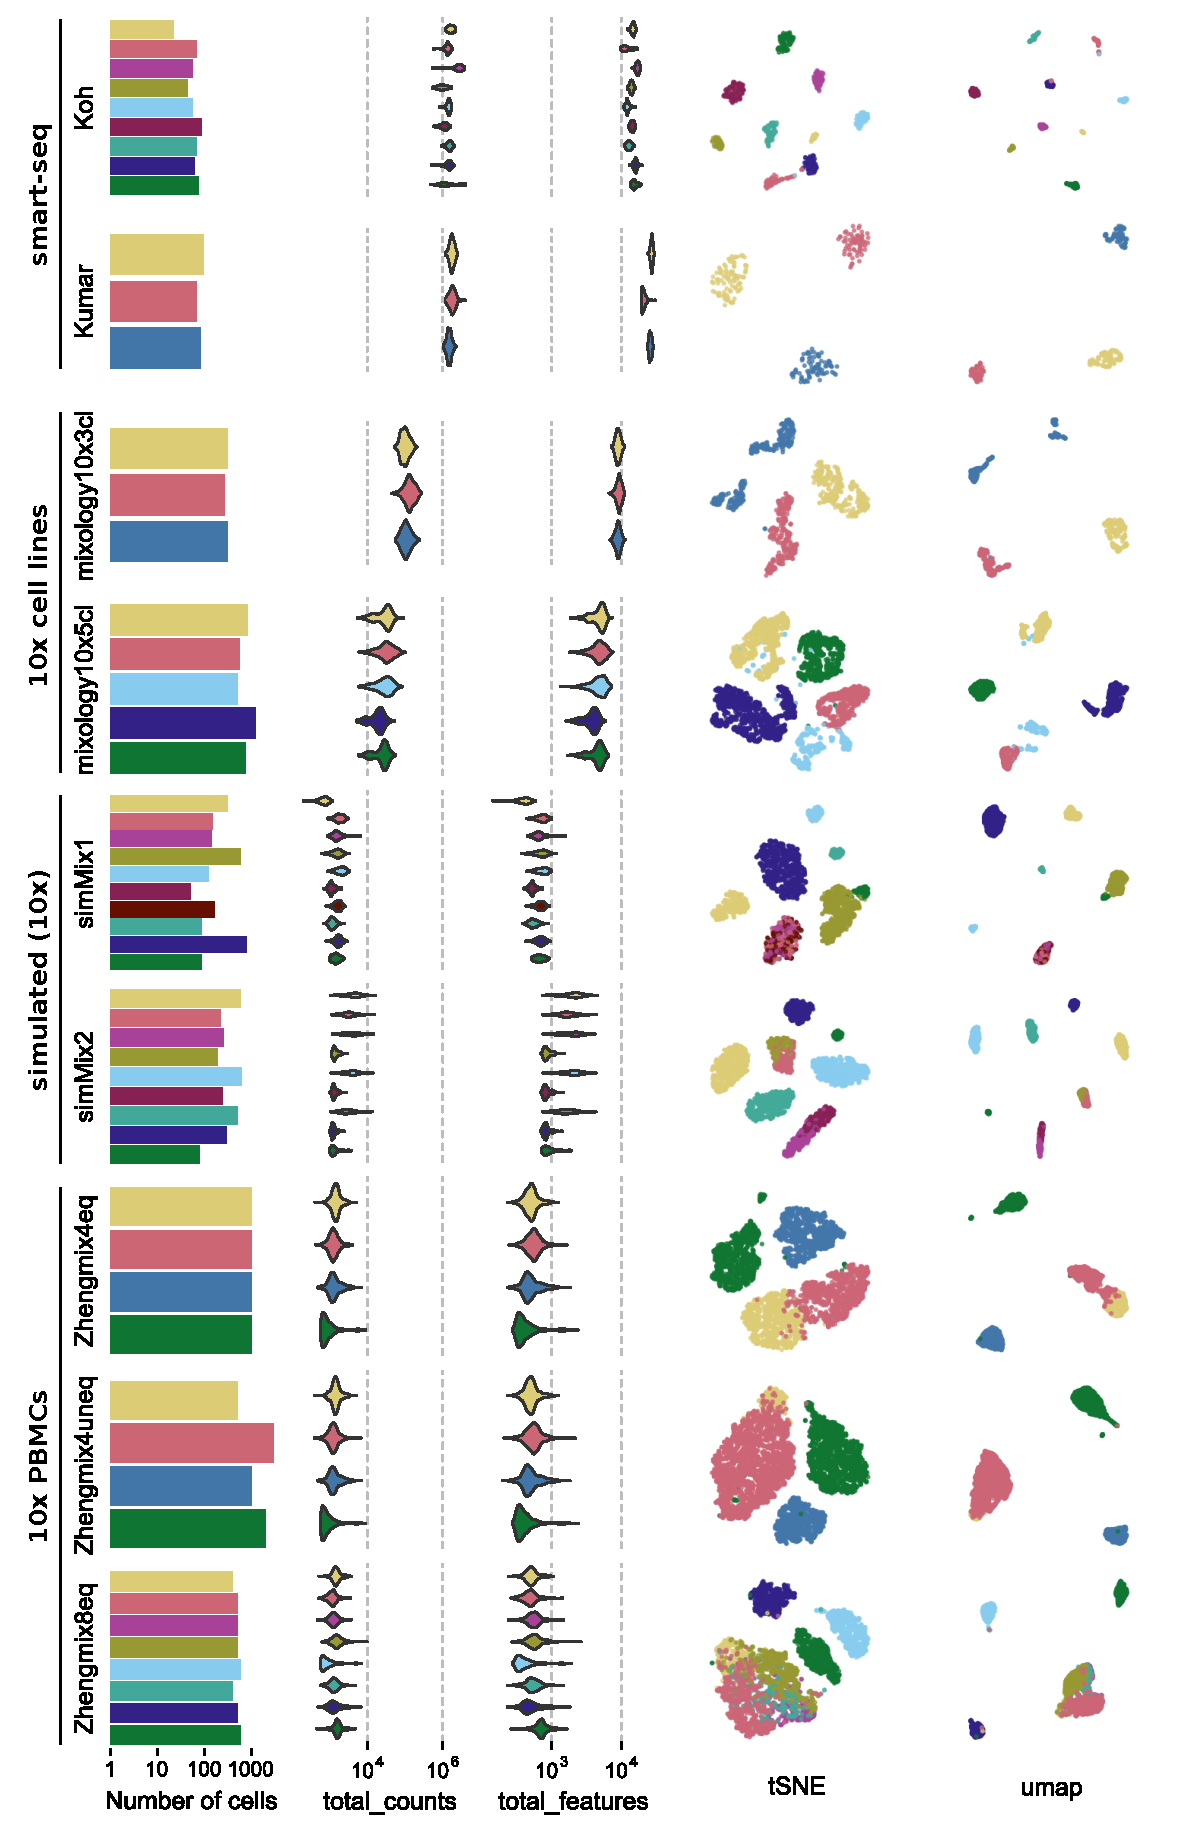
\includegraphics[width=\textwidth,keepaspectratio]{dataset_description}
    \caption{\textbf{Overview of the benchmark datasets used.}}
    \label{fig:figure1}
\end{figure}

\begin{figure}
    \centering
    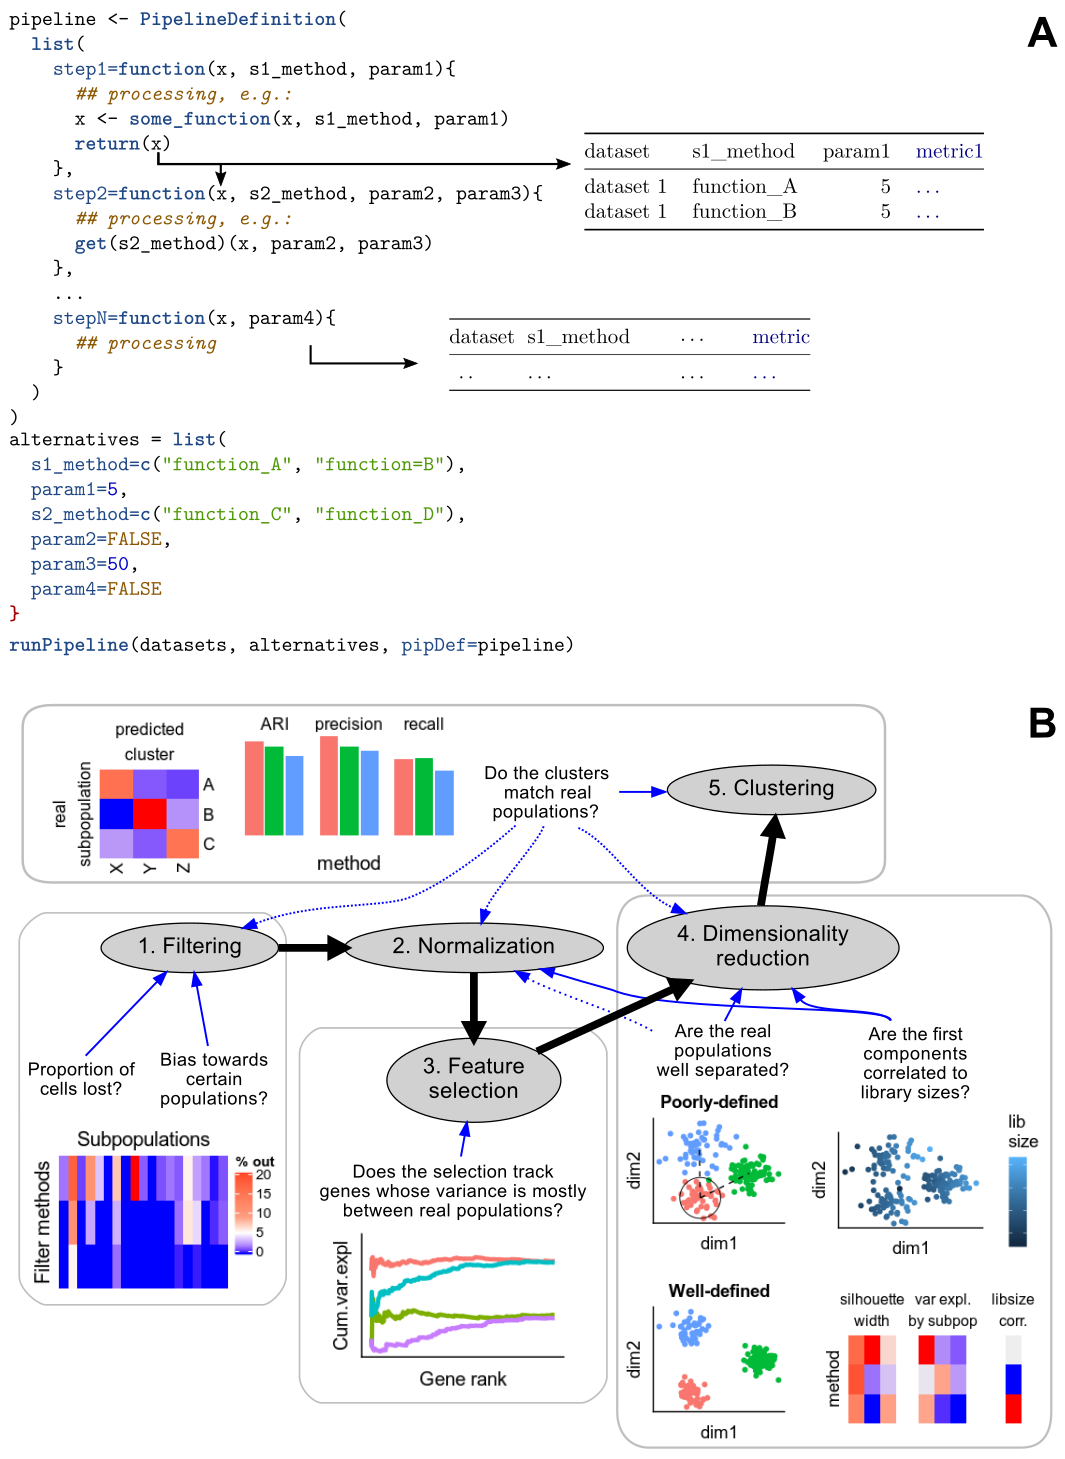
\includegraphics[width=\textwidth,keepaspectratio]{main_figures/pipeline_explanation.png}
    \caption{\textbf{Overview of the pipeComp framework and its application to a scRNAseq clustering pipeline.}}
    \label{fig:figure2}
\end{figure}

\subsection*{Filtering}

\subsubsection*{Doublet detection}

Doublets, defined as two cells sequenced under the same cellular barcode (e.g., being captured in the same droplet), are fairly frequent in scRNAseq datasets, with estimates ranging from 1 to 10\% depending on the platform and cell concentration used \citep{bloomEstimating2018,kangMultiplexedDemuxlet2018}. While doublets of the same cell type are relatively innocuous for most downstream applications due to their conservation of the relative expression between genes, doublets formed from different cell types or states are likely to be misclassified and could potentially distort downstream analysis. In some cases, doublets can be identified through their unusually high number of reads and detected features, but this is not always the case (Supplementary Figure 2). A number of methods were developed to identify doublets, in most cases by comparing each cell to artificially-created doublets \citep{mcginnisDoubletfinder2019, LunScran2016, BaisScds2019}. We therefore first evaluated the capacity of these methods to detect doublets using the two 10x datasets with cells of different genetic identity \citep{tianMixology2018}, and for which therefore SNP information can be used as ground truth. We included a further such dataset\citep{kangMultiplexedDemuxlet2018} not included for the rest of our benchmark due to the absence of true cell labels beside SNPs. Of note, SNP-based analyses also call doublets created by cells of the same cell type (but from different individuals), whose identification is generally not the primary aim of doublet detection methods, since these can be considered homotypic (as opposed to neotypic or heterotypic doublets, i.e. doublets from different cell types) and can be identified through other means.

We tested \textit{DoubletFinder} \citep{mcginnisDoubletfinder2019} and \textit{scran}'s \texttt{doubletCells} \citep{LunScran2016}, both of which use similarity to artificial doublets, and \textit{scds} \citep{BaisScds2019}, which relies on a combination of co-expression and binary classification. \textit{DoubletFinder} integrates a thresholding based on the proportion of expected doublets, while \textit{scran} and \textit{scds} return scores that must be manually thresholded. In these cases, we ensured that the right number of cells would be called doublets. In addition to these methods, we reasoned that an approach such as \textit{DoubletFinder} could be simplified by being applied directly on counts and by using a pre-clustering to create neotypic/heterotypic doublets more efficiently. We therefore developed a simple and fast Bioconductor package implementing this method for doublet detection, \textit{scDblFinder}, with the added advantage of accounting for uncertainty in the expected doublet rate and using meta-cells from the clusters to even include triplets (see methods).

While most methods accurately identified the doublets in the 3 cell lines dataset (mixology10x3cl), the other two datasets proved more difficult (Figure \ref{fig:figure3}A). \textit{scDblFinder} achieved comparable or better accuracy than top alternatives while running in a very reasonable time (Figure \ref{fig:figure3}B). Across datasets, cells called as doublets tended to be classified in the wrong cluster more often than other cells (Figure \ref{fig:figure3}C. We therefore tested whether this method also improved the accuracy of the clustering across all benchmark datasets, and found that it did even when, by design, the data contained no heterotypic doublet (Figure \ref{fig:figure4}).

\begin{figure}
    \centering
    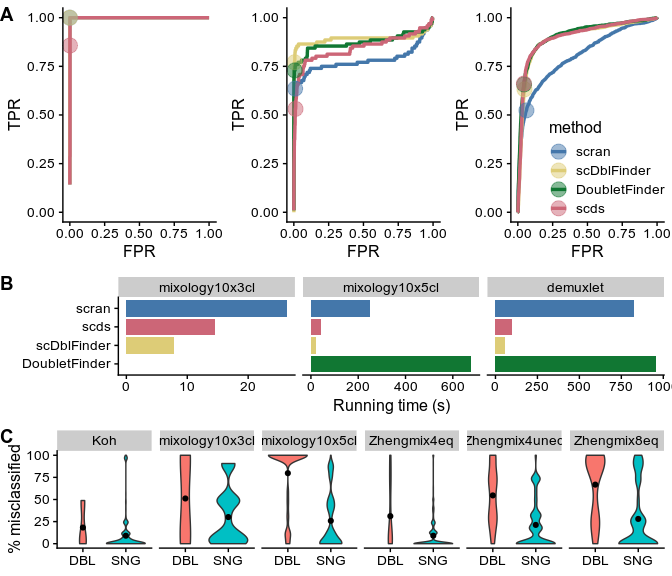
\includegraphics[width=\textwidth]{{main_figures/doublets_files/figure-html/figure1-1.png}}
    \caption{\textbf{Identification of doublet cells. A:} Receiver operating characteristic (ROC) curves of the tested doublet detection methods for three datasets with SNP-identified doublets. Dots indicate threshold determined by the true number of doublets. \textbf{B:} Running time of the different methods (DoubletFinder failed on one of the datasets). \textbf{C:} Rate of misclassification of the cells identified by \textit{scDblFinder} as doublets (DBL) or singlets (SNG), across a large range of clustering analysis. Even in datasets which should not have neotypic doublets, the cells identified as such tend to be misclassified.    \label{fig:figure3}}
\end{figure}

\subsubsection*{Excluding more cells is not necessarily better}

Beyond doublets, a dataset might include low-quality cells whose elimination would reduce noise. This has for instance been demonstrated for droplets containing a high content of mitochondrial reads, often as a result of cell degradation and resulting loss of cytoplasmic mRNAs \citep{IlicicLowQual2016}. A common practice is to exclude cells that differ considerably from most other cells on the basis of such properties, for instance through the \texttt{isOutlier} function of \textit{scater} that measures, for a given control property, the number of median absolute deviations of each cell from the median of all cells. Supplementary Figure 1 shows the distributions of some of the typical cell properties commonly used. Of note, these properties tend to be correlated, with some exceptions. For instance, while a high proportion of mitochondrial reads is often correlated with a high proportion of the counts in the top features, there can also be other reasons for an over-representation of highly-expressed features (Supplementary Figure 3), such as an over-amplification in non-UMI datasets. In our experience, 10X datasets also exhibit a very strong correlation between the total counts and the total features even across very different cell types (Supplementary Figure 4). We therefore also measure the ratio between the two, and treat cells strongly departing from this trend with suspicion.

Reasoning that the cells we wish to eliminate are cells that would be misclassified, we measured the rate of misclassification of each cell in each dataset across a variety of clustering pipelines, correcting for the median misclassification rate of the subpopulation, and then evaluated what properties could be predictive of misclassification (Supplementary Figures 5-7). We could not identify any property or simple combination thereof that would be consistently predictive of misclassification; the only feature that consistently stood out across multiple datasets (the Zheng datasets) was that cells with very high read counts have a higher chance of being misclassified.

We next investigated the impact of filtering according to various criteria (see methods). An important risk of excluding cells on the basis of their distance from the whole distribution of cells on some properties (e.g. library size) is that these properties tend to have different distributions across subpopulations. As a result, thresholds in terms of number of median absolute deviations (MADs) from the whole distribution can lead to strong biases against certain subpopulations (Figure \ref{fig:figure4}A). We therefore examined the tradeoff between the increased accuracy of filtering and the maximum proportion of cells excluded per subpopulation (Figure \ref{fig:figure4}B and Supplementary Figure 8). Since filtering changes the relative abundance of the different subpopulations, global clustering accuracy metrics such as ARI are not appropriate here, and we therefore calculated the per-subpopulation precision and recall using the Hungarian algorithm \citep{PapadimitriouHu1998}, and monitored their mean F1 score. A first observation was that, although the stringent filtering tended to be associated with an increase in accuracy, it could also become deleterious, and most of the benefits could be achieved without very stringent filtering and minimizing subpopulation bias. Applying the same filtering criteria on individual clusters of cells (identified through scran's \texttt{quickCluster} method) resulted in nearly no cell being filtered out. This suggests that filtering on the global population tends to discard cells of subpopulations with more extreme properties (e.g. high library size), rather than low-quality cells. Finally, by changing the distributions, the doublet removal step in conjunction with filtering sometimes resulted in a net decrease in the proportion of excluded cells while retaining or improving accuracy. We therefore recommend the use of doublet removal followed by relatively mild filtering, such as is implemented in our `default' filtering (see methods).

\begin{figure}
    \centering
    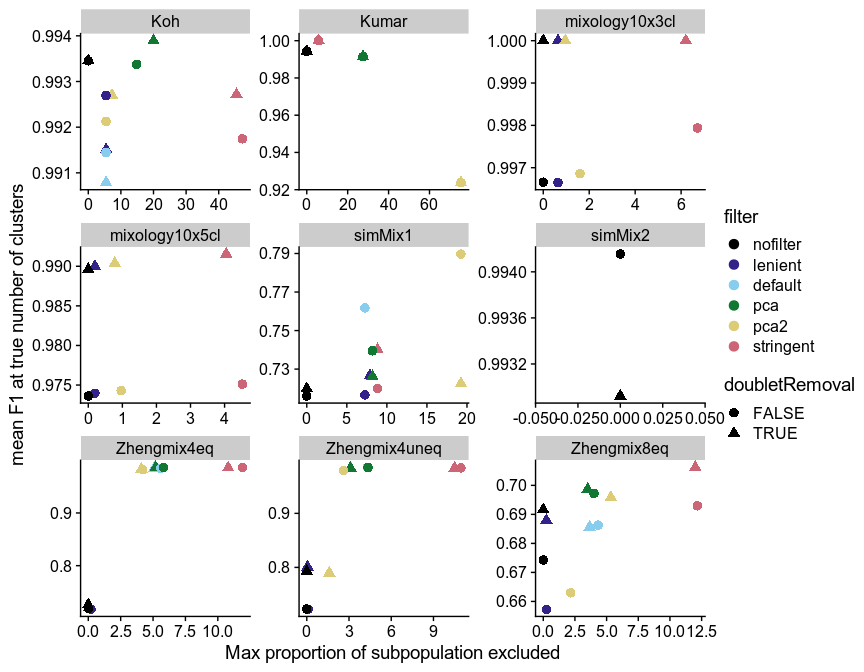
\includegraphics[width=\textwidth]{{main_figures/filtering_files/figure-html/figure2-1.png}}
    \caption{\textbf{A:} Filtering on the basis of distance to the whole distribution can lead to strong bias against certain subpopulations. The dashed line indicates a threshold of 2.5 median absolute deviations (MADs) from the median of the overall population. \textbf{B:} Relationship between the maximum subpopulation exclusion rate and the average clustering accuracy per subpopulation across various filtering strategies. Of note, doublet removal appears to be desirable even when, due to the design, there are no heterotypic doublets in the data. The PCA methods refer to multivariate outlier detected as implemented in \textit{scater} (see methods for details).}
    \label{fig:figure4}
\end{figure}

\subsubsection*{Filtering features by type}

Mitochondrial reads have been associated with cell degradation and there is evidence that ribosomal genes can influence the clustering output, hiding other biological structure in the analysis \citep{freytagComparison2018}. We therefore investigated whether excluding one category of features or the other, or using only protein-coding genes, had an impact on the ability to distinguish subpopulations (Supplementary Figure 9). Removal of ribosomal genes robustly reduced the quality of the clustering, suggesting that they represent real biological differences between subpopulations. Removing mitochondrial genes and restricting to protein-coding genes had a very mild impact.

\subsection*{Normalization and scaling}

We next investigated the impact of different normalization strategies. Beside the standard log-normalization included in \textit{Seurat}, we tested \textit{scran}'s pooling-based normalization \citep{lunPooling2016}, \textit{sctransform}'s variance-stabilizing transformation \citep{hafemeisterSCtransform2019}, and normalization based on stable genes \citep{linStableGenes2018, deekeStablyExpressed2018}. 
In addition to log-normalization, the standard \textit{Seurat} clustering pipeline performs per-feature unit-variance scaling so that the PCA is not too strongly dominated by highly-expressed features. We therefore included versions of the different normalization procedures, with or without a subsequent scaling (\textit{sctransform}'s variance-stabilizing transformation involves something analogous to scaling). 
\textit{Seurat}'s scaling function also includes the option to regress out the effect of certain covariates. We tested its performance by using the proportion of mitochondrial counts and the number of detected features as covariates. Finally, it has been proposed that the use of stable genes, in particular cytosolic ribosomal genes, can be used to normalize scRNAseq\citep{deekeStablyExpressed2018}. We therefore evaluated a simple linear normalization based on the sum of these genes, as well as nuclear genes.

An important motivation for the development \textit{sctransform} was the observation that, even after normalization, the first principal components of various datasets tended to correlate with library size, suggesting an inadequate normalization \citep{hafemeisterSCtransform2019}. We therefore first assessed to what extent the first principal component still retained a correlation with the library size and the number of detected features, removing the confounding covariation with the subpopulations (Figure \ref{fig:figure5}A). The simple step of scaling tended to remove much of the correlation with these features and, in the absence of scaling, standard \textit{Seurat} normalization resulted in fairly high correlation with technical covariates. \textit{sctransform} led to the lowest correlation but most methods, including normalization based on stable genes, were able to remove most of the correlation when combined with scaling. The only exception is \textit{Seurat} normalization with scaling regressing out covariates, which surprisingly increased the correlation in 8 of the 9 datasets.

We next investigated the impact of normalization on the separability of the subpopulations (Figure \ref{fig:figure5}B-C). Since clustering accuracy metrics such as the ARI are very strongly influenced by the number of clusters, we complemented it with silhouette width\citep{RousseeuwSil1987} and mutual information. We found most methods (including no normalization at all) to perform fairly well in most of the subpopulations. Scaling tended to reduce the average silhouette width of some subpopulations and to increase that of some less distinguishable ones, and was generally but not always beneficial on the accuracy of the final clustering. Regressing out covariates systematically gave poorer performance on all metrics. \textit{sctransform} systematically outperformed other methods, and even though it was developed to be applied to data with unique molecular identifiers (UMI), it also performed fairly well with Smart-seq protocol (Koh and Kumar datasets).

\begin{figure}
    \centering
    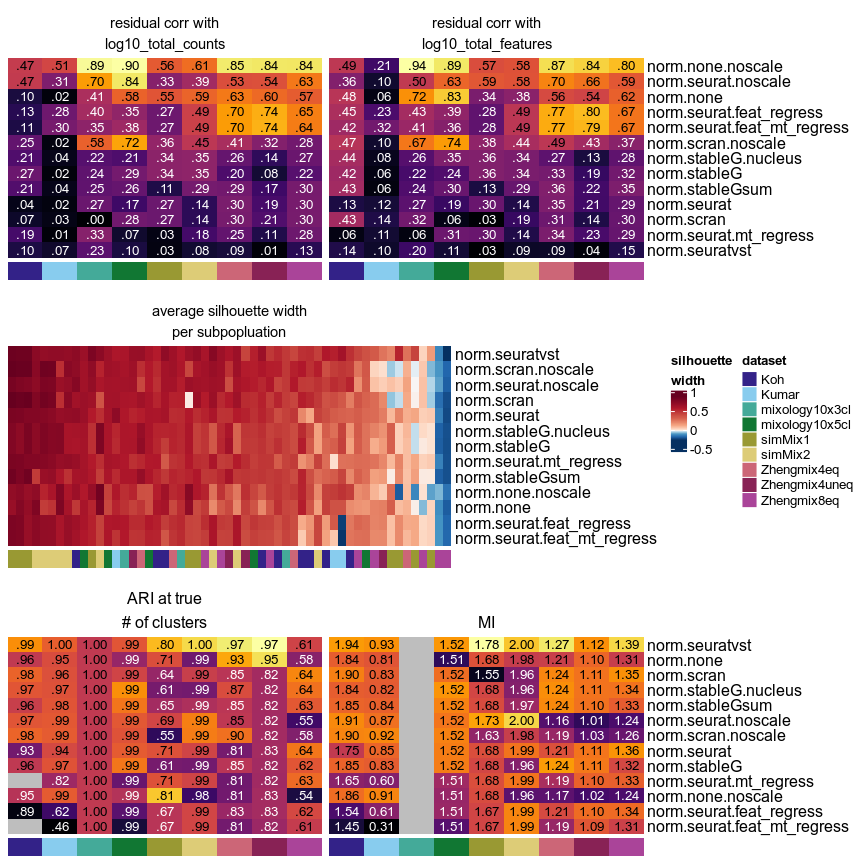
\includegraphics[width=\textwidth]{{main_figures/normalization_files/figure-html/figure3-1.png}}
    \caption{\textbf{Evaluation of normalization procedures.} `Seurat.feat\_mt\_regress' indicates the regressing out of the number of features and proportion of mitochondrial reads during scaling, represents, and `Seurat.feat\_regress` of the number of features only.  Residual correlation of the first principal component with library size (left) and detection rate (right), after accounting for biological differences between subpopulations. \textbf{B:} Average silhouette width per true subpopulation, where higher silhouette width means a higher separability. \textbf{C:} Clustering accuracy, measured by the ARI at the true number of cluster (left) and by the average mutual information (MI) of the cluster assignment with true subpopulations.}
    \label{fig:figure5}
\end{figure}

Finally, we monitored whether, under the same downstream clustering analysis, different normalization methods tended to lead to an over- or under-estimation of the number of clusters. Although some methods had a tendency to lead to a higher (e.g. \textit{sctransform}) or lower (e.g. stable genes) number of clusters, the effect was very mild and not entirely systematic (Supplementary Figure 10).

\subsection*{Feature selection}

A standard clustering pipeline typically involves a step of highly-variable genes selection, which is complicated by the digital nature and the mean-variance relationship of (sc)RNAseq. \textit{Seurat}'s earlier approaches involved the use of dispersion estimates standardized for the mean expression levels, while more recent versions (>3) rely on a different measure of variance, again standardized. Of note, while adjusting for the mean-variance relationship removes much of the bias towards highly-expressed genes, it is plausible that this relationship may in fact sometimes reflects biological relevance and would be helpful in classifying cell types. Another common practice in features selection is to use those with the highest mean expression, and recently, \citep{townesGlmpca2019} instead suggested to use deviance, while \textit{sctransform} provides its own ordering of genes based on transformed variance.

Reasoning that a selection method should ideally select genes whose variability is more between subpopulations than within, we first assessed to what extent each method selected genes with a high proportion of variance or deviance explained by (real) subpopulation. As the proportion of variability in a gene attributable to subpopulations can be measured in various ways, we first compared three such alternatives. Analysis of variance performed on a standard \textit{Seurat} normalization or on \textit{sctransform} data were highly correlated (Supplementary Figure 11A). These estimates were also in good agreement with the deviance explained, although lowly-expressed genes could have a high deviance explained without having much of their variance explained by subpopulation (Supplementary Figure 11B-D). We therefore compared the proportion of the cumulative variance/deviance explained by the top X genes that could be retrieved by each gene ranking method (Supplementary Figures 12-13). We first focused on the first 1000 genes to highlight the differences between methods, although a higher number of selected genes decreased the differences between methods (Supplementary Figures 12-14). The standardized measures of variability were systematically worse than their non-standardized counterparts in selecting genes with a high proportion of variance explained by subpopulation. Regarding to the percentage of deviance explained however, the standardized measures were often superior(Figure \ref{fig:figure6}A and Supplementary Figures 12-13). Deviance proved the method of choice to prioritize genes with a high variance explained by subpopulations (with mere expression level proving surprisingly good), but did not perform so well to select genes with a high deviance explained.

\begin{figure}
    \centering
    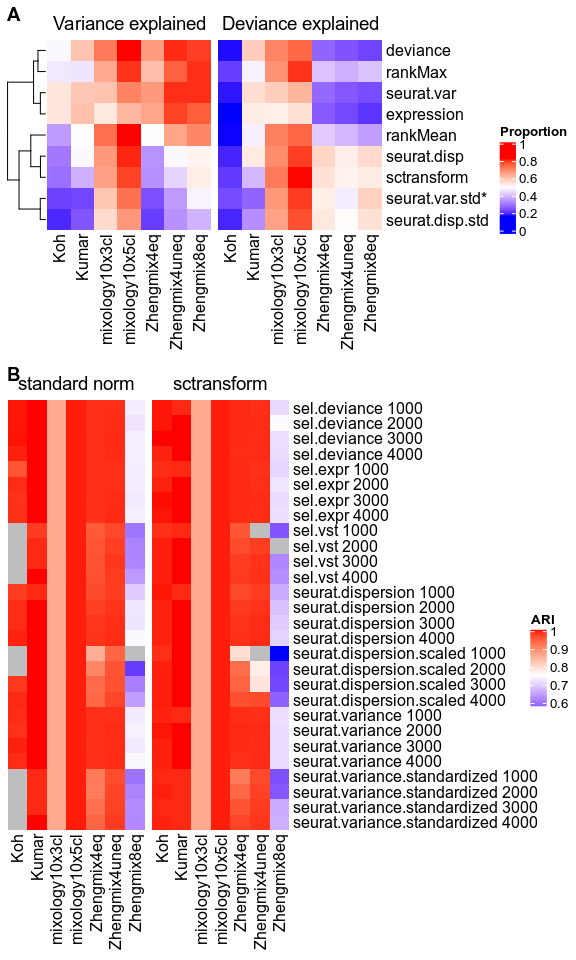
\includegraphics[scale=0.6]{{main_figures/selection_files/figure-html/figure4-1.png}}
    \caption{\textbf{Evaluation of feature selection methods. A:} Ability of different feature ranking methods to capture genes with a high proportion of variance (left) or deviance (right) explained by real subpopulations. The asterix denotes the default Seurat method. \textbf{B:} Accuracy of clusterings (at the true number of clusters) when selecting 1000 genes using the given methods. Based on standard \textit{Seurat} normalization (left) or \textit{sctransform} (right). The methods `vst.varExp' and `devianceExplained' are the estimates used in \textbf{A} to evaluate the selection methods, and were included here only for validation purpose.}
    \label{fig:figure6}
\end{figure}

We next evaluated how the use of different feature selection methods affected the clustering accuracy (Figure \ref{fig:figure6}B). To validate the previous assay on the proportion of variance/ deviance explained by real populations, we included genes that maximized these two latter measures. Interestingly, while these selections were on average the top-ranking methods, they were not systematically best for all datasets. The previous observations were reflected in the ARI of the resulting clustering (Figure \ref{fig:figure6}B): non-standardized measures of variability, including mere expression level, tended to outperform more complex metrics. In general, we found deviance and unstandardized estimates of variance to provide the best results across datasets and normalization methods. Increasing the number of features selected also systematically led to an increase in the accuracy of the clustering, typically plateauing after 4000 features (Supplementary Figure 14).

\subsection*{Dimensionality reduction}

We next investigated the methods of dimensionality reduction. Since the various PCA approaches and implementations were recently benchmarked in a similar context \citep{TsuyuzakiPCA2020}, we focused on widely used approaches which had not yet been compared: \textit{Seurat}'s PCA, \textit{scran}'s \texttt{denoise PCA}, and GLM-PCA \citep{townesGlmpca2019}, and combined them (when relevant) with \textit{sctransform} normalization. Given that \textit{Seurat}'s default PCA weights the cell embeddings by the variance of each component, we also evaluated the impact of this weighting with each method.

The impact of the choice of dimensionality reduction method was far greater than that of normalization or feature selection (e.g. Supplementary Figure 15). The first components identified by GLM-PCA tended to have a higher proportion of their variance explained by real subpopulations and increase the average silhouette width of already well-defined subpopulations. Seurat's PCA procedure however proved superior on all metrics (Figure \ref{fig:figure7}). 
Overall, weighting the principal components by their variance in the same fashion as Seurat's method does had a strong positive impact on silhouette widths and ARI scores.

\begin{figure}
    \centering
    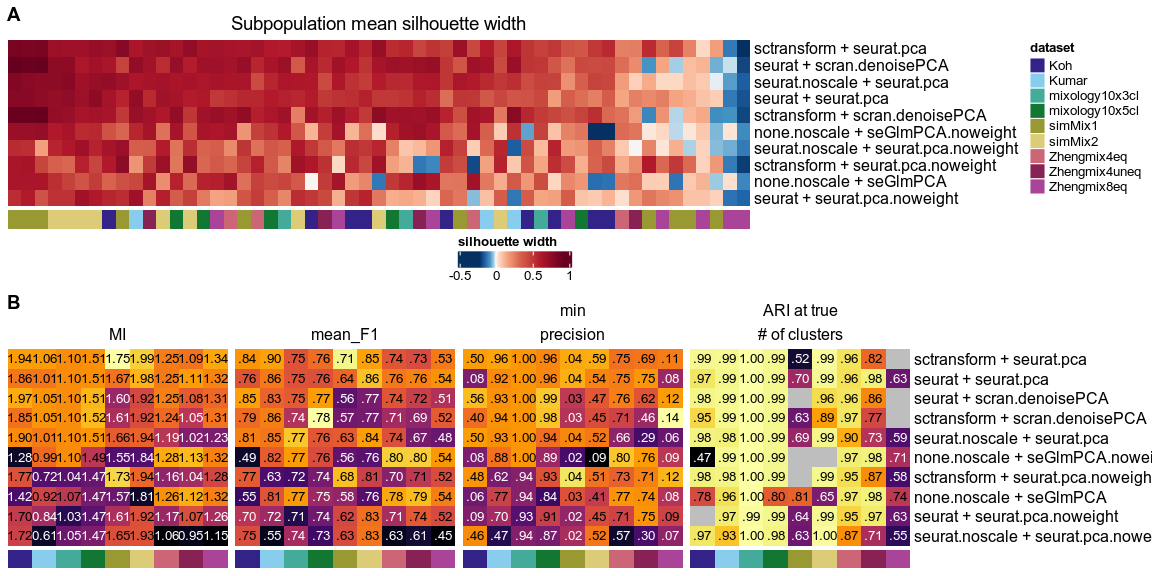
\includegraphics[width=\textwidth]{{main_figures/dr_files/figure-html/dimred-1.png}}
    \caption{\textbf{Evaluation of common dimensionality reduction methods. A:} Average silhouette width per subpopulation resulting from combinations of normalization and dimension reductions. \textbf{B:} Clustering accuracy , mean proportion of the variance in the first 5 components explained by real subpopulations (center), and median ARI of the resulting clustering (right).}
    \label{fig:figure7}
\end{figure}

\subsubsection*{Estimating the number of dimensions}

A common step following dimension reduction is the selection of an appropriate number of dimensions to use for downstream analysis. Since euclidean distance decreases as the number of non-discriminating dimensions increases, there is usually a trade-off between selecting enough dimensions to keep most information and excluding smaller dimensions that may represent technical noise or other unwanted sources of variation. Overall, increasing the number of dimensions robustly led to a decrease in the number of clusters (Supplementary Figures 15). This tended to be translated to the accuracy of the clustering (Supplementary Figure 16), although in both cases (number of clusters and ARI) \textit{Seurat}'s resolution parameter had a much stronger impact.

Different approaches have been proposed to select the appropriate number of dimensions, from the visual identification of an 'Elbow' (inflexion point) of the variance explained, to more complex algorithms. We evaluated the performance of common tools, namely [TBD] (\textit{pcaLocal.FO} label, [REF needed?]), global maximum likelihood based on translated Poisson Mixture Model (\textit{maxLikGlobal}, \citep{haroTranslated2008}), [TBD] (\textit{essLocal.b}, \textit{essLocal.b},[REF needed?]), JackStraw procedure (\textit{jackstraw.elbow}, \citep{ChungJackstraw2015}), [TBD](\textit{pcaLocal.maxgap}, [REF needed?]), [TBD] (\textit{pcaLocal.fan} [REF needed?]), Fisher Separability analysis (\textit{fisherSeparability}, \citep{AlberganteSepar2019}), \textit{scran}'s \texttt{denoisePCA} function (\textit{scran.denoisePCA}, \citep{LunScran2016}) and [TBD] (\textit{pcaOptmPointwise.max}, [REF needed?]).

We compared the various estimates of dimensionality in their ability to retrieve the intrinsic number of dimensions in a dataset, based on Seurat's weighted PCA space. As a first approximation of the true dimensionality, we computed the variance in each principal component that was explained by the subpopulations, which sharply decreased after the first few components in most datasets (Figure \ref{fig:figure8}A). Figure \ref{fig:figure8}B shows the difference between the dimension estimates of the above methods and that based on the subpopulations (i.e. from Figure \ref{fig:figure8}A). Of note, the methods differ widely in view of their computing time (Figure \ref{fig:figure8}B) and we saw no relationship between the accuracy of the estimates and the complexity of the method. Reasoning that over-estimating the number of dimensions is less problematic than under-estimating it, we kept the former methods for a full analysis of their impact on clustering (Figure \ref{fig:figure8}C-D), when combined with sctransform or the standard Seurat normalization. Although most methods performed well on the various clustering measures, the global maximum likelihood based on translated Poisson Mixture Model (\textit{maxLikGlobal}) provided the dimensionality estimate that best separated the subpopulations (Figure \ref{fig:figure8}C) and resulted in the best clustering accuracy (Figure \ref{fig:figure8}D). This method systematically selected many more components than were associated with the subpopulations, suggesting that although these additional components appear individually uninformative, in combination they nevertheless contribute to classification.

\begin{figure}
    \centering
    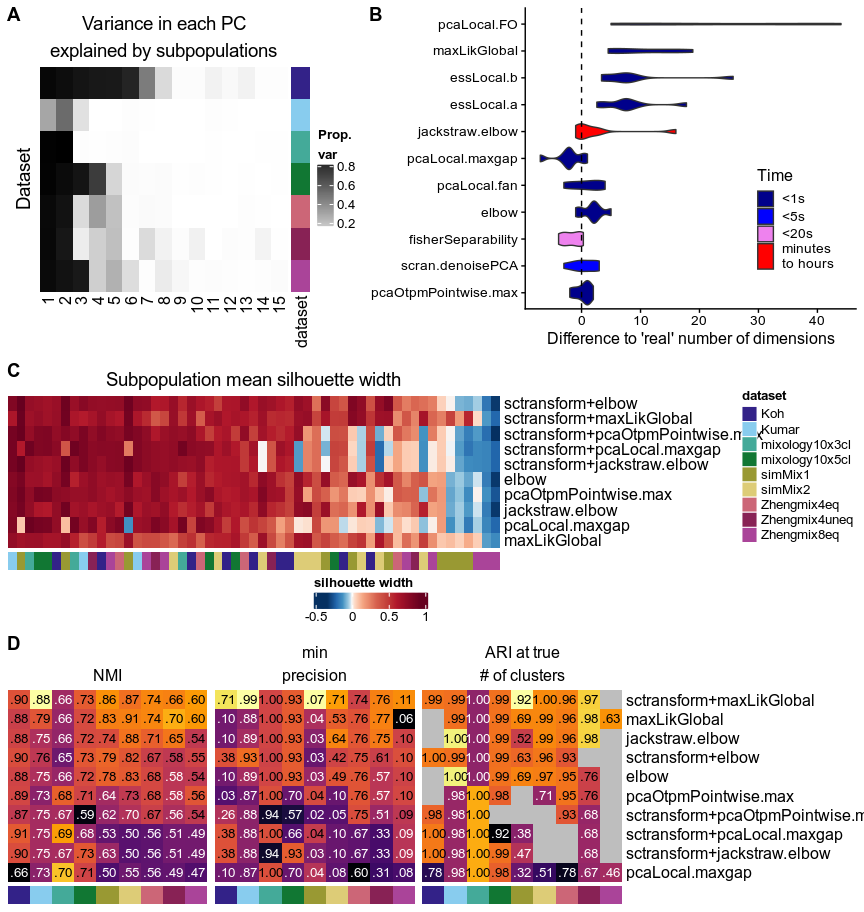
\includegraphics[width=\textwidth]{{main_figures/dimensionality_files/figure-html/figure6-1.png}}
    \caption{\textbf{Estimating dimensionality. A:} Estimated dimensionality using the proportion of variance in each component explained by the true subpopulations. \textbf{B:} Difference between `real' dimensionality (from \textbf{A}) and dimensionality estimation methods, along with computing time. \textbf{C:} Average silhouette width per subpopulation across a selection of methods, combined with \textit{sctransform} or standard \textit{Seurat} normalization. \textbf{D:} Clustering accuracy across the normalization/dimensionality estimation methods.}
    \label{fig:figure8}
\end{figure}

\subsection*{Clustering}

The last step evaluated in our pipeline was clustering. Given previous works on the topic \citep{duoClustering2018,freytagComparison2018} and the success of graph-based clustering methods for scRNA-seq, we restricted our evaluation to Seurat's method and two \textit{scran} SNN-based clustering approaches, based on random walks (\textit{walktrap} method) or on the optimization of the modularity score (\textit{fast\_greedy}). Again, the tested methods were combined with Seurat's standard normalization and \textit{sctransform}, otherwise using the parameters found optimal in the previous steps. 

Since ARI is dominated by differences in the number of clusters, and no single metric is perfect, we diversified them (Figure \ref{fig:figure9}). Mutual information (MI) has the virtue of not decreasing when a true subpopulation is split into two clusters, which is arguably less problematic (and might well reflect unknown biological subgroups), but as a consequence it can be biased towards methods producing higher resolution clustering. Similarly, precision per true subpopulation is considerably more robust to differences in the number of clusters. We also tracked the mean F1 score and the ARI at the true number of clusters. 

The MI score and minimum precision, which are largely independent of the estimated number of clusters, were overall higher for the walktrap method (Figure \ref{fig:figure9}), while the mean F1 score favored both \textitt{scran} methods (walktrap and fast greedy) over \textit{Seurat}. Finally, the ARI score at the true number of clusters, when available, showed similar performances. However, while \textit{Seurat}'s resolution parameter had a large impact on the number of clusters identified, and therefore could be used to find a parameter combination producing the right number of clusters, the number of clusters found by \textit{scran}-based clustering was considerably less influenced by the available parameters (number of nearest neighbors or steps in the random walk - see Supplementary Figure 17). The occasional lack of scran-based clustering with the right number of clusters, along with a higher mutual information, suggest that \textit{scran} sometimes simply divides a real subpopulation into two (possibly tracking some unknown biological differences) rather than committing misclassification errors. Overall, the walktrap method appeared superior to the fast greedy algorithm and was generally less prone to misclassification than \textit{Seurat} clustering, although the latter offered more control over the resolution. Of note, very difficult subpopulations, both from the Zhengmix8eq and simMix1 datasets, remained very inaccurately classified by all methods and in regards to all metrics.


\begin{figure}
    \centering
    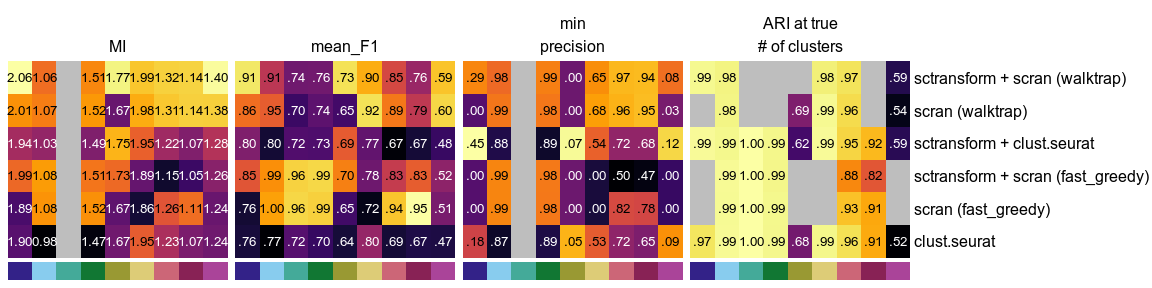
\includegraphics[width=\textwidth]{{main_figures/clustering_files/figure-html/clustering-1.png}}
    \caption{\textbf{Evaluation of clustering methods.} Clustering accuracy of common clustering tools in combination with \textitt{sctransform} and standard Seurat's normalization.}
    \label{fig:figure9}
\end{figure}

\subsection*{Further extensions to the pipeline: imputation/denoising}

The basic pipeline presented here can be extended with additional analysis steps while keeping the same evaluation metrics. To demonstrate this, we evaluated various imputation or denoising techniques based on their impact on classification. As preliminary analysis showed that all methods performed equally well or better on normalized data, we applied them after filtering and normalization, but before scaling and reduction. Although some of the methods (e.g. \textit{DRImpute\_process} and \textit{alra\_norm}) did improve the separability of some more elusive subpopulations, no method had a systematically positive impact on the average silhouette width across all subpopulations (Figure \ref{fig:figure10}A). When restricting ourselves to clustering analyses that yielded the `right' number of clusters, all tested methods improved classification  compared to a scenario with no imputation step (`none' label, Figure \ref{fig:figure10}B). However, the situation was not so straightforward with alternative metrics, where some methods (e.g. \textit{enhance}) consistently underperformed. 10X datasets, which are typically characterized by a lower per-cell coverage and feature detection rate, expectedly benefited more from imputation, and in this context \textit{DRImpute} and \textit{dca} tended to show the best performance. On the contrary, imputing on normalized counts originating from Smart-seq technology was instead rather deleterious to the clustering accuracy. Our recommendation follows the previous benchmarking of imputation strategies performed by \citep{ZhangImput2018}. Although this previous study focused on trajectory inference and preservation of data structure as main metrics, \textit{DrImpute} also revealed to be among the top performers and was recommended for clustering analysis (\textit{alra} was however not included in this previous evaluation).


\begin{figure}
    \centering
    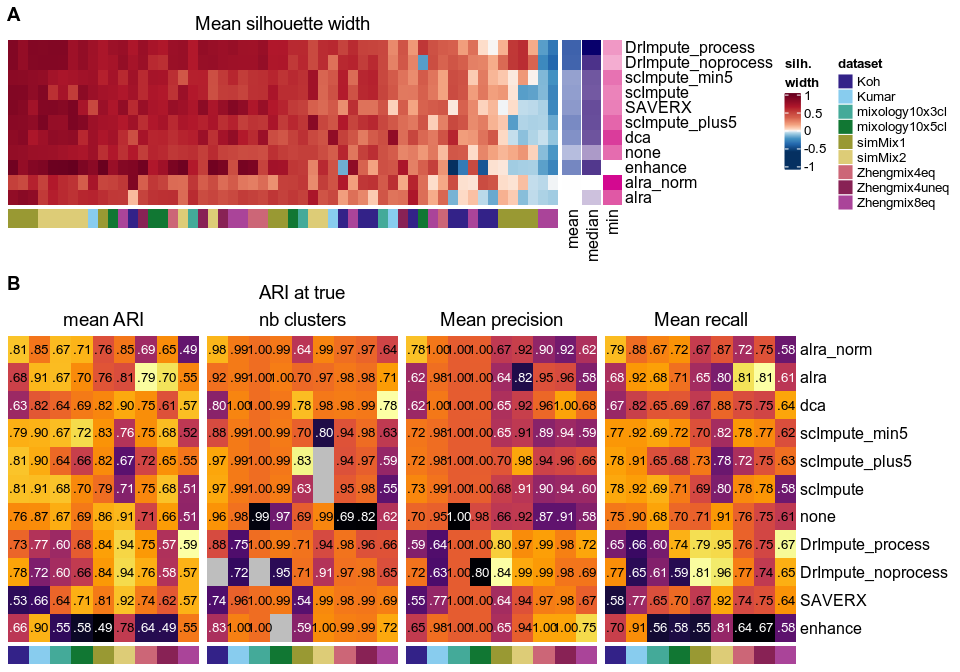
\includegraphics[width=\textwidth]{{main_figures/imputation_files/figure-html/imputation-1.png}}
    \caption{\textbf{Imputation/denoising methods} Average silhouette width per subpopulation (\textbf{A}) and clustering accuracy (\textbf{B}) with or without (\textit{none}) application of a denoising/imputation method}
    \label{fig:figure10}
\end{figure}


\section*{Discussion}

\subsection*{Concrete recommendations}

On the basis of our findings, we can make a number of concrete analysis recommendations:

\begin{enumerate}
   \item Filtering
   \begin{itemize}
     \item Doublet detection and removal is advised, and can be performed at little computing cost with software such as \textit{scDblFinder} or \textit{scds}.
     \item Distribution-based cell filtering fails to capture doublets, and should use relatively lenient cutoffs (e.g. 5 MADs, or 3 MADs in at least 2 distributions) to exclude poor-quality cells while avoiding bias.
     \item Features filtering based on feature type did not appear beneficial.
   \end{itemize}
   \item Normalization and scaling
   \begin{itemize}
     \item Most normalization methods tested yielded a fair performance, especially when combined with scaling, which tended to have a positive impact on clustering.
     \item \textit{sctransform} offered the best overall performance in terms of the separability of the subpopulations, as well as removing the effect of library size and detection rate.
     \item The common practice of regressing out cell covariates such as the detection rate or proportion of mitochondrial reads nearly always had a negative impact, leading to increased correlation with covariates and decreased clustering accuracy. We therefore advise against this practice.
   \end{itemize}
   \item Feature selection
   \begin{itemize}
     \item Deviance \citep{townesGlmpca2019} offered the best ranking of genes for feature selection.
     \item Increasing the number of features included tended to lead to better classifications, plateauing from 4000 features.
   \end{itemize}
   \item Denoising/imputation
   \begin{itemize}
       \item Denoising appeared beneficial to the identification of subpopulations in 10x datasets, but not in Smart-seq datasets.
       \item We found especially \textit{alra} (with prior normalization), \textit{DrImpute} (with prior processing) and \textit{dca} to offer the best performances.
   \end{itemize}
   \item PCA
   \begin{itemize}
     \item Similarly to previous reports \citep{SunDimRed2019}, we recommend the irlba-based PCA using weighting of the components, as implemented in \textit{Seurat}. 
     \item Instead of the common elbow or jackstraw methods for deciding on the components to include, we recommend the \textit{global maximum likelihood based on translated Poisson Mixture Model} method (e.g. implemented in \texttt{intrinsicDimension::maxLikGlobalDimEst()}).
   \end{itemize}
   \item Clustering
   \begin{itemize}
    \item We found \textit{scran}-based walktrap clustering to show good performances.
    \item In cases where prior knowledge can guide the choice of a resolution, \textit{Seurat} can be useful in affording manual control of it while, in the absence of such knowledge, \textit{scran}-based walktrap clustering provided reasonable estimates.
   \end{itemize}
\end{enumerate}



\subsection*{Limitations and open questions}

In this study, we evaluated tools commonly used for the processing of scRNAseq with a focus on droplet-based datasets, namely from the 10x technology. Although this platform has been used in almost half of the scRNAseq studies in 2019 \citep{SvenssonDB2019}, other popular technologies such as Drop-seq, InDrops or Smart-seq2/3 were not represented in the present benchmarking. Differences between such protocols have a very large impact on clustering \citep{MereuCellAtlas2019}. Although most top-ranking methods in our comparison performed well on both Smart-seq and 10x datasets that we tested, future benchmarking efforts should strive to include less represented technologies. In addition, we did not compare any of the alignment and/or quantification methods used to obtain the count matrix \citep{MereuCellAtlas2019}. Some steps, such as the implementation of the PCA step, were also not explored in detail here as they have already been the object of recent and thorough study elsewhere \citep{SunDimRed2019}. We also considered only methods relying on Euclidean distance, while correlation was recently reported to be superior\citep{kim_impact_2019} and would require further investigation.

Here, we chose to concentrate on what could be learned from datasets with known cell labels (as opposed to labels inferred from the data, as in \citep{MereuCellAtlas2019}). In contrast to \citep{tianMixology2018}, who relied on RNA mixtures of known proportions, we chose to rely chiefly on real cells and their representative form of variability. Given the limited availability of such datasets however, several aspects of single-cell analysis could not be compared, such as batch effect correction or multi-dataset integration. In addition, a focus on the identification of the subpopulations might fail to reveal methods which are instead best performing for tasks other than clustering, such as differential expression analysis or trajectory inference. Some informative benchmarks have already been performed on some of these topics \citealp{SaelensTraject2019, SonesonDE2018}. Yes, such evaluations could benefit from considering methods not in isolation, but as parts of a connected workflow, as we have done here. We believe that the \textit{pipeComp} framework is modular and flexible enough to integrate new steps in the pipeline, as it was shown as an example with the evaluation of imputation/ denoising methods.

We believe there is much space for improvement in methods. Concerning cell filtering, we noticed that the current approach based on whole-population characteristic (e.g. MAD cut-off) can be biased against certain subpopulations, suggesting that more refined methods expect multimodal distributions could be used rather than relying on whole-population characteristics. In addition, most common filtering approaches do not harness the relationship between cell QC properties. Finally, imputation had a varied impact on the clustering analysis and seemed to be linked to the technology that was used to generate the data. We support the hypothesis of \citep{ZhangImput2018} on the respective strengths of linear models and non-linear models and their use to different types of data, such as the performance of non-linear methods in developmental studies. 

\section*{Conclusions}

\textit{pipeComp} is a flexible R framework for evaluating methods and parameter combinations in a complex pipeline, computing on-the-fly multilevel evaluation metrics. Application of this framework to scRNAseq clustering enabled us to make concrete recommendations on the steps of filtering, normalization, feature selection, denoising, dimensionality reduction and clustering. We show a diversity of multilevel metrics to be more robust, more sensitive, and more nuanced than simply evaluating the final clustering. In addition, we provide a new, efficient Bioconductor package for doublet detection. Finally, we hope that the \textit{pipeComp} framework can be applied to extend the current benchmark, as well as to apply it to other contexts.

\section*{Methods}

\subsection*{Code and data availability}

All analyses were performed through the \href{https://github.com/plger/pipeComp}{pipeComp} R package, which implements the pipeline framework described here. All code to reproduce the simulations and figures is available in the \url{https://github.com/markrobinsonuzh/scRNA\_pipelines\_paper} repository, which also includes the basic datasets with a standardized annotation.

The gene counts for the two mixology datasets were downloaded from the  \href[CellBench repository]{https://github.com/LuyiTian/CellBench\_data/data/sincell\_with\_class.RData}, commit 74fe79e. For the other datasets, we used the unfiltered counts from \citep{duoClustering2018}, available on the corresponding repository \url{https://github.com/markrobinsonuzh/scRNAseq\_clustering\_comparison}. For simplicity, all starting \textit{SingleCellExperiment} objects with standardized metadata are available on \url{https://github.com/markrobinsonuzh/scRNA\_pipelines\_paper}.

\subsection*{Software and package versions}
Analyses were performed in R 3.6.0 (Bioconductor 3.9), and the following packages were installed from github repositories: \textit{Seurat} (version 3.0.0), \textit{sctransform} (0.2.0), \textit{DoubletFinder} (2.0.1), \textit{scDblFinder} (1.1.1), \textit{scds} (1.0.0), \textit{SAVERX} (1.0.0), \textit{scImpute} (0.0.9), \textit{ALRA} (commit 7636de8), \textit{DCA} (0.2.2), \textit{DrImpute} (1.2), \textit{ENHANCE} (R version, commit 1571696), \textitt{SAVERX} (1.0.0). The code for the glmPCA was obtained from \url{https://github.com/willtownes/scrna2019} (commit 1ddcc30ebb95d083a685f12fe81d35dd1b0cb1b2).

\subsection*{Simulated datasets}
The simMix1 dataset was based on the human PBMC CITE-seq data deposited under accession code GSE100866 of the Gene Expression Omnibus (GEO) website. Both RNA and ADT count data were downloaded from GEO and processed independently using \textit{Seurat}. We then considered cells that were in the same cluster both in the RNA-based and ADT-based analyses to be real subpopulations, and focused on the 4 most abundant ones. We then performed 3 sampling-based simulations with various degrees of separation using \textit{muscat} \citep{CrowellMuscat2019}, and merged the three simulations. The simMix2 dataset was generated from the mouse brain data published in \cite{CrowellMuscat2019} in a similar fashion. The specific code is available on \url{https://github.com/markrobinsonuzh/scRNA\_pipelines\_paper}.

\subsection*{Default pipeline parameters}

Where unspecified, the following default parameters or parameter sets were used:
\begin{itemize}
    \item \textit{scDblFinder} was used for doublet identification
    \item the default filter sets (see below) were applied
    \item standard \textit{Seurat} normalization was employed
    \item \textit{Seurat} (v3) variable feature selection was employed, selecting 2000 genes
    \item standard \textit{Seurat} scaling and PCA were employed
    \item To study the impact of upstream steps on clustering, various \textit{Seurat} clustering analyses were performed, selecting different numbers of dimensions (5, 10, 15, 20, 30, and 50) and using various resolution parameters (0.005, 0.01, 0.02, 0.05, 0.1, 0.15, 0.2, 0.3, 0.4, 0.5, 0.8, 1, 1.2, 1.5, 2, 4). The range of resolution parameters was selected to ensure that the right number of clusters could be obtained in all datasets.
\end{itemize}

\subsubsection{Denoising/imputation}
Most imputations/ denoising methods were run with the default parameters with the following exceptions; \textit{DrImpute} documentation advises to process the data prior to imputation by removing lowly expressed genes and cells expressing less than 2 genes. As it is not clear if this step is a hard requirement for the method to perform well, \textit{DrImpute} was run with and without prior processing (\textit{DrImpute\_process} and \textit{DrImpute\_noprocess} labels, respectively). \textit{dca} method does not accept non-integers counts but two of the datasets being used contain such table of counts due to multimapping. For these datasets, we rounded up the counts prior to imputation. \textit{alra} is designed for normalized data but as we are evaluating normalization downstream to imputation, we used the method on both non-normalized (\textit{alra} label) and normalized counts (\textit{alra\_norm} label). \textit{scImpute} requires an estimation of the expected number of clusters with the input data. As the estimation of the true number of cluster may not be known by the user, we evaluated the tool using the true number of clusters (\textit{scImpute} label) and using an over/under-estimation of this number (\textit{scImpute\_plus5} and \textit{scImpute\_min5} labels, respectively). \textit{ENHANCE} uses a k-nearest neighbor aggregation method and automatically estimates the number of neighbors to merge prior to the imputation. With the smallest datasets that we used, this lead to an early stop of the function as this parameters was estimated to 1. In such cases, we manually set this parameter to 2 for the method to work. 

\subsection*{Doublet detection method}
Our doublet detection method is available at \url{https://github.com/plger/scDblFinder}. Briefly, after reducing the data to the most expressed genes, we cluster the cells using the fast-greedy algorithm, favouring overclustering. We then create artificial doublets by sampling the two cells specifically from different clusters, and sum the counts of each pair of cells. We also create meta-cells from each cluster, and use them to create additional doublets and triplets. We combine them with the real cells, perform PCA and build a KNN graph using \textit{BiocNeighbors}. We then calculate, for each cell, the proportion of its neighbors that are artificial doublets, weighted by the distance. This ratio serves as a doublet score, which is then thresholded by simultaneously minimizing the error in classifying real vs artificial doublets and the deviation from the distribution of expected doublet rate (accounting for homotypic doublets as done by \textit{DoubletFinder}).

\subsection*{Filter sets}
The \textit{default} set of filters excludes cells that are outliers according to at least two of the following thresholds: log10\_total\_counts $>$2.5 MADs or $<$5 MADs, log10\_total\_features $>$2.5 MADs or $<$5 MADs, pct\_counts\_in\_top\_20\_features $>$ or $<$ 5 MADs, featcount\_dist (distance to expected ratio of log10 counts and features) $>$ or $<$ 5 MADs, pct\_counts\_Mt $>$ 2.5 MADs and $>$ 0.08.

The \textit{stringent} set of filters uses the same thresholds, but excludes a cell if it is an outlier on any single distribution. 

The \textit{lenient} set of filters excludes cells that are outliers on at least two distributions by at least 5 MADs, except for pct\_counts\_Mt where the threshold is $>$ 3 MADs and $>$ 0.08.

For cluster-wise filters, clusters were first identified with \textit{scran::quickCluster} and the filters were then applied separately for each cluster. 

The `pca' and `pca2' clusters refer to the multivariate outlier detection methods implemented in \textit{scater}, running \textit{runPCA} with \texttt{use\_coldata=TRUE, detect\_outliers=TRUE}. `pca` uses all covariates, while `pca2` uses only the log10(counts), log10(features), proportion mitochondrial and proportion in the top 50 features.

\subsection*{Variance and deviance explained}

Unless specified otherwise, the variance in gene expression explained by subpopulations was calculated on the data normalized and transformed through \textit{sctransform}. For each gene, we fitted a linear model using the subpopulation as only independent variable (\textasciitilde subpopulation), and used the R-squared as a measure of the variance explained. The same method was used for principal components.

The deviance explained by subpopulations was calculated directly on counts using the \texttt{pipeComp::getDevianceExplained} function. The function uses \textit{edgeR} to fit two models, a full \textasciitilde librarySize+subpopulation model and a reduced \textasciitilde librarySize model. For each gene, the deviance explained is then the difference between the deviance of each models, divided by the deviance of the reduced model. In the rare cases where this resulted in a negative deviance explained, it was set to zero.

To estimate the correlation between the principal components and covariates such as library size, we first fitted a linear model on the subpopulations, and correlated the residuals of this model with the covariate of interest.


%%%%%%%%%%%%%%%%%%%%%%%%%%%%%%%%%%%%%%%%%%%%%%
%%                                          %%
%% Backmatter begins here                   %%
%%                                          %%
%%%%%%%%%%%%%%%%%%%%%%%%%%%%%%%%%%%%%%%%%%%%%%

\begin{backmatter}

\section*{Competing interests}
  The authors declare that they have no competing interests.

\section*{Author's contributions}
    Text for this section \ldots

\section*{Acknowledgements}
  Text for this section \ldots
%%%%%%%%%%%%%%%%%%%%%%%%%%%%%%%%%%%%%%%%%%%%%%%%%%%%%%%%%%%%%
%%                  The Bibliography                       %%
%%                                                         %%
%%  Bmc_mathpys.bst  will be used to                       %%
%%  create a .BBL file for submission.                     %%
%%  After submission of the .TEX file,                     %%
%%  you will be prompted to submit your .BBL file.         %%
%%                                                         %%
%%                                                         %%
%%  Note that the displayed Bibliography will not          %%
%%  necessarily be rendered by Latex exactly as specified  %%
%%  in the online Instructions for Authors.                %%
%%                                                         %%
%%%%%%%%%%%%%%%%%%%%%%%%%%%%%%%%%%%%%%%%%%%%%%%%%%%%%%%%%%%%%

% if your bibliography is in bibtex format, use those commands:
\bibliographystyle{bmc-mathphys} % Style BST file (bmc-mathphys, vancouver, spbasic).
\bibliography{bmc_article}      % Bibliography file (usually '*.bib' )
% for author-year bibliography (bmc-mathphys or spbasic)
% a) write to bib file (bmc-mathphys only)
% @settings{label, options="nameyear"}
% b) uncomment next line
%\nocite{label}

% or include bibliography directly:
% \begin{thebibliography}
% \bibitem{b1}
% \end{thebibliography}

%%%%%%%%%%%%%%%%%%%%%%%%%%%%%%%%%%%
%%                               %%
%% Figures                       %%
%%                               %%
%% NB: this is for captions and  %%
%% Titles. All graphics must be  %%
%% submitted separately and NOT  %%
%% included in the Tex document  %%
%%                               %%
%%%%%%%%%%%%%%%%%%%%%%%%%%%%%%%%%%%

%%
%% Do not use \listoffigures as most will included as separate files

% \section*{Figures}
%   \begin{figure}[h!]
%   \caption{\csentence{Sample figure title.}
%       A short description of the figure content
%       should go here.}
%       \end{figure}
% 
% \begin{figure}[h!]
%   \caption{\csentence{Sample figure title.}
%       Figure legend text.}
%       \end{figure}

%%%%%%%%%%%%%%%%%%%%%%%%%%%%%%%%%%%
%%                               %%
%% Tables                        %%
%%                               %%
%%%%%%%%%%%%%%%%%%%%%%%%%%%%%%%%%%%

%% Use of \listoftables is discouraged.
%%
\section*{Tables}

\begin{table}[h!]
\caption{Overview of the benchmark datasets}
\label{tab:table1}
\begin{tabular}{rlrrl}
  \hline
dataset & source & protocol & description \\ 
  \hline
Koh & GSE85066 & SMARTer & FACS purified H7 hESC in different differention stages \\ 
  Kumar & GSE60749 & SMARTer & Mouse ESC cultured in different conditions \\ 
  Zhengmix4eq & \citep{duoClustering2018} & 10x & Mixtures of FACS purified PBMCs \\ 
  Zhengmix4uneq & \citep{duoClustering2018} & 10x & Mixtures of FACS purified PBMCs \\ 
  Zhengmix8eq & \citep{duoClustering2018} & 10x & Mixtures of FACS purified PBMCs \\ 
  mixology10x3cl & \cite{tianMixology2018} & 10x & Mixture of 3  cancer cell lines from CellBench \\ 
  mixology10x5cl & \cite{tianMixology2018} & 10x & Mixture of 5 cancer cell lines from CellBench \\ 
  simMix1 & - & 10x-based & Simulation of 10 human cell subpopulations \\
  simMix2 & - & 10x-based & Simulation of 9 mouse cell subpopulations \\
   \hline
\end{tabular}
\end{table}

%%%%%%%%%%%%%%%%%%%%%%%%%%%%%%%%%%%
%%                               %%
%% Additional Files              %%
%%                               %%
%%%%%%%%%%%%%%%%%%%%%%%%%%%%%%%%%%%

\section*{Additional Files}
  \subsection*{Supplementary figures}
    % Additional file descriptions text

\end{backmatter}
\end{document}
